% !TEX spellcheck = en_US



% ~~~~~~~~~~~~~~~~~~~~~~~~~~~~~~~~~~~~~~~ V
% (NC) 2026 Haluk Bingol
% github.com/halukbingol/LaTeX-Templates
%
% Licensees may copy, distribute, display, and perform the work and make derivative works 
% and remixes based on it only for non-commercial purposes. 
% ~~~~~~~~~~~~~~~~~~~~~~~~~~~~~~~~~~~~~~~ A




% =====================================================================
%  Queues -- The Concepts
%  ---------------------------------------------------------------------
%  Built on hblib/Template/hblibTemplate.tex with the libraries in ../../hblib/.
%  The only program here is a jshell session in codeoutput/.
% =====================================================================

\documentclass[aspectratio=169,10pt,compress]{beamer}

% ~~~~~~~~~~~~~~~~~~~~~~~~~~~~~~~~~~~~~~~~~~~~~~~~~~~~~~~~~~~~~~~~~ V hblib
	\usepackage{../../hblib/hblibPresentation} % lib presentation: theme, i/N, \hSection, algorithm2e, ...
	\usepackage{../../hblib/hblibCodeoutput} % lib code + output: \lstcode, \lstterminal, ...
	\usepackage{../../hblib/hblibDatastructures} % lib data structures: \hString, \hStack, \hQueue
% ~~~~~~~~~~~~~~~~~~~~~~~~~~~~~~~~~~~~~~~~~~~~~~~~~~~~~~~~~~~~~~~~~ A hblib


% xcolor, array (and the L{width} column), listings, tikz and algorithm2e come from the hblib libraries
\usepackage[T1]{fontenc}
\usepackage{lmodern}
\usepackage{booktabs}

\newcommand{\win}{\textbf{Windows}}
\newcommand{\mac}{\textbf{macOS}}

% listings: fixed character cells, so the columns of a program's output stay aligned
\lstset{columns=fixed}

% algorithm2e set-up (the package is loaded by hblibPresentation)
\SetAlCapFnt{\small}
\SetAlCapNameFnt{\small}
\SetKwProg{Fn}{function}{}{end}
\SetKw{KwError}{error}

% ---------------------------------------------------------------------
\title{Queues}
\subtitle{The Concepts}
\author[Bingol]{Ruhan Alpaydin}

\institute[FCIS]{
    Faculty of Computer and Information Sciences\\
    Yeditepe University
}
\date{
	{\tiny \hbTimeStamp}
}

\begin{document}




% ~~~~~~~~~~~~~~~~~~~~~~~~~~~~~~~~~~~~~~ V frm
\begin{frame}[t,fragile]
  \titlepage
\end{frame}
% ~~~~~~~~~~~~~~~~~~~~~~~~~~~~~~~~~~~~~~ A frm




% ~~~~~~~~~~~~~~~~~~~~~~~~~~~~~~~~~~~~~~ V frm
\begin{frame}[t,fragile] \frametitle{Outline}
  \begin{columns}[T]
    \begin{column}{0.48\textwidth}
      \tableofcontents[sections={1-4}, hideallsubsections]
    \end{column}
    \begin{column}{0.48\textwidth}
      \tableofcontents[sections={5-8}, hideallsubsections]
    \end{column}
  \end{columns}
\end{frame}
% ~~~~~~~~~~~~~~~~~~~~~~~~~~~~~~~~~~~~~~ A frm

% ~~~~~~~~~~~~~~~~~~~~~~~~~~~~~~~~~~~~~~ V
\hSection[Idea]{The Idea of a Queue}
% ~~~~~~~~~~~~~~~~~~~~~~~~~~~~~~~~~~~~~~ A

% ~~~~~~~~~~~~~~~~~~~~~~~~~~~~~~~~~~~~~~ V
\subsection[FIFO]{First in, first out}
% ~~~~~~~~~~~~~~~~~~~~~~~~~~~~~~~~~~~~~~ A




% ~~~~~~~~~~~~~~~~~~~~~~~~~~~~~~~~~~~~~~ V frm
\begin{frame}[t,fragile] \frametitle{A queue of people}
  \begin{columns}[T]
    \begin{column}{0.4\textwidth}
      \begin{center}
        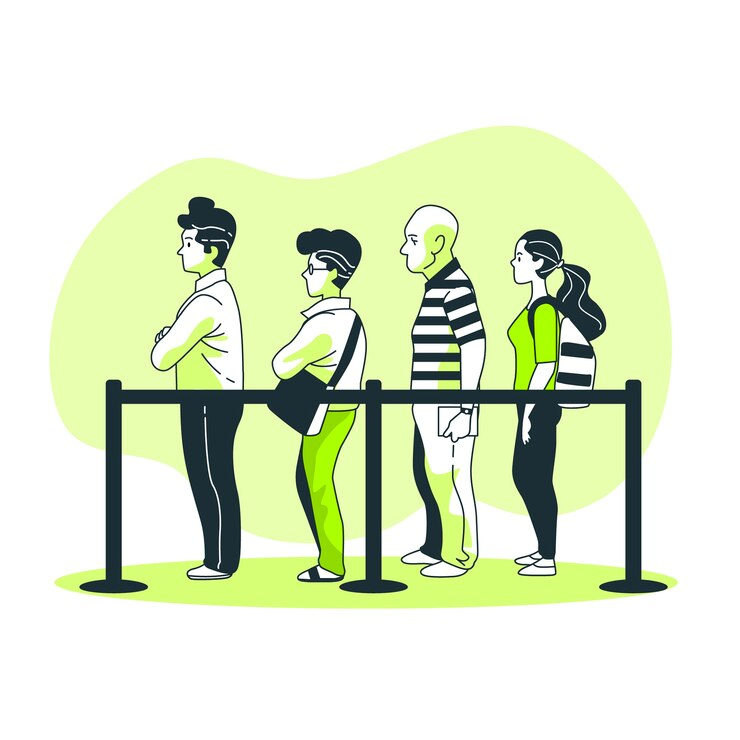
\includegraphics[width=\textwidth]{fig-queuePeople.jpg}
      \end{center}
    \end{column}
    \begin{column}{0.56\textwidth}
      \begin{itemize}
        \item A newcomer joins at the \textbf{rear}.
        \item The next person is served at the \textbf{front}.
        \item Nobody in the middle leaves first: \hRemark{first in, first out}.
        \item The line can be long or short, but the order never changes.
      \end{itemize}
      \begin{block}{Definition}
        A \textbf{queue} is a collection where insertion happens at one end,
        the \textbf{rear}, and removal at the other end, the \textbf{front}.
      \end{block}
    \end{column}
  \end{columns}
\end{frame}
% ~~~~~~~~~~~~~~~~~~~~~~~~~~~~~~~~~~~~~~ A frm




% ~~~~~~~~~~~~~~~~~~~~~~~~~~~~~~~~~~~~~~ V frm
\begin{frame}[t,fragile] \frametitle{First in, first out}
  \begin{columns}[T]
    \begin{column}{0.5\textwidth}
      \begin{center}\footnotesize
      \begin{tabular}{lll}
        \toprule
        \textbf{Operation} & \textbf{Returns} & \textbf{Queue} \\
        \midrule
        \texttt{enqueue(A)} &      & A \\
        \texttt{enqueue(B)} &      & A B \\
        \texttt{enqueue(C)} &      & A B C \\
        \texttt{dequeue()}  & A    & B C \\
        \texttt{enqueue(D)} &      & B C D \\
        \texttt{peek()}     & B    & B C D \\
        \texttt{dequeue()}  & B    & C D \\
        \bottomrule
      \end{tabular}
      \end{center}
    \end{column}
    \begin{column}{0.46\textwidth}
      \begin{block}{FIFO}
        The element that has waited the longest is served first:\\
        \hRemark{First In, First Out}.
      \end{block}
      \small
      Compare with a stack: last in, first out. Same elements, same arrival order,
      \hRemark{opposite order of leaving}.
    \end{column}
  \end{columns}
\end{frame}
% ~~~~~~~~~~~~~~~~~~~~~~~~~~~~~~~~~~~~~~ A frm




% ~~~~~~~~~~~~~~~~~~~~~~~~~~~~~~~~~~~~~~ V frm
\begin{frame}[t,fragile] \frametitle{Queues around us}
  \begin{center}\small
  \begin{tabular}{L{0.27\textwidth}L{0.29\textwidth}L{0.34\textwidth}}
    \toprule
    \textbf{Where}              & \textbf{enqueue}                        & \textbf{dequeue} \\
    \midrule
    A ticket line               & a new customer arrives                  & the clerk calls the next one \\
    A printer                   & a document is sent to print             & the printer starts a document \\
    The keyboard buffer         & a key is pressed                        & the program reads a key \\
    The operating system        & a program becomes ready                 & the CPU runs it for a while \\
    A call centre               & a call starts waiting                   & an operator becomes free \\
    A network router            & a packet arrives                        & the link is free: send it \\
    A message queue             & a producer publishes a message          & a consumer handles it \\
    \bottomrule
  \end{tabular}
  \end{center}
  \vspace{0.4em}
  In every case the oldest unfinished item is handled first, and \textbf{arrival order} is the fairness rule.
\end{frame}
% ~~~~~~~~~~~~~~~~~~~~~~~~~~~~~~~~~~~~~~ A frm




% ~~~~~~~~~~~~~~~~~~~~~~~~~~~~~~~~~~~~~~ V frm
\begin{frame}[t,fragile] \frametitle{Queue vs stack}
  \begin{columns}[T]
    \begin{column}{0.48\textwidth}
      \begin{block}{Stack: LIFO}
        \begin{center}
        \begin{tikzpicture}\hStack{0}{6}{3}{A,B,C,D}[0.55][0.45]\end{tikzpicture}
        \end{center}
        \small Insert and remove at the \textbf{same} end (the top). \texttt{pop} gives \textbf{D}.
      \end{block}
    \end{column}
    \begin{column}{0.48\textwidth}
      \begin{block}{Queue: FIFO}
        \begin{center}
        \begin{tikzpicture}\hQueueArray{6}{0}{4}{4}{A,B,C,D}[0.55][0.45]\end{tikzpicture}
        \end{center}
        \small Insert at the rear, remove at the front. \texttt{dequeue} gives \textbf{A}.
      \end{block}
    \end{column}
  \end{columns}
  \vspace{0.6em}
  \small The same four elements, added in the same order, leave in \hRemark{opposite} orders.
\end{frame}
% ~~~~~~~~~~~~~~~~~~~~~~~~~~~~~~~~~~~~~~ A frm

% ~~~~~~~~~~~~~~~~~~~~~~~~~~~~~~~~~~~~~~ V
\hSection[ADT]{The Queue ADT}
% ~~~~~~~~~~~~~~~~~~~~~~~~~~~~~~~~~~~~~~ A

% ~~~~~~~~~~~~~~~~~~~~~~~~~~~~~~~~~~~~~~ V
\subsection[Operations]{Operations}
% ~~~~~~~~~~~~~~~~~~~~~~~~~~~~~~~~~~~~~~ A




% ~~~~~~~~~~~~~~~~~~~~~~~~~~~~~~~~~~~~~~ V frm
\begin{frame}[t,fragile] \frametitle{What a queue can do}
  \begin{center}\small
  \begin{tabular}{lL{0.4\textwidth}L{0.32\textwidth}}
    \toprule
    \textbf{Operation}    & \textbf{Meaning}                                  & \textbf{If the queue is \dots} \\
    \midrule
    \texttt{enqueue(x)}   & add \texttt{x} at the rear                        & full: \hRemark{overflow} \\
    \texttt{dequeue()}    & remove the front element and return it            & empty: \hRemark{underflow} \\
    \texttt{peek()}       & return the front element, do not remove it        & empty: \hRemark{underflow} \\
    \texttt{isEmpty()}    & is there no element?                              & -- \\
    \texttt{size()}       & number of elements                                & -- \\
    \bottomrule
  \end{tabular}
  \end{center}
  \vspace{0.5em}
  \begin{itemize}\small
    \item This list is an \textbf{abstract data type} (ADT): it says \emph{what} a queue does, not \emph{how}.
    \item \texttt{peek} is also called \texttt{front}. Overflow exists only if the capacity is fixed.
  \end{itemize}
\end{frame}
% ~~~~~~~~~~~~~~~~~~~~~~~~~~~~~~~~~~~~~~ A frm




% ~~~~~~~~~~~~~~~~~~~~~~~~~~~~~~~~~~~~~~ V frm
\begin{frame}[t,fragile] \frametitle{Rules every queue obeys}
  For any queue $Q$ and element $x$:
  \[
  	\texttt{peek}(\texttt{enqueue}(Q, x)) = x
  \]
  \[
  	\texttt{dequeue}(\texttt{enqueue}(Q, x)) \text{ returns } x \text{ and leaves } Q
  \]
  \[
  	\texttt{size}(\texttt{enqueue}(Q, x)) = \texttt{size}(Q) + 1
  \]
  \[
  	\texttt{isEmpty}(Q) \iff \texttt{size}(Q) = 0
  \]
  \vspace{0.3em}
  \begin{itemize}\small
    \item Any implementation (circular array, linked list, \dots) must make these true.
    \item They are also good \textbf{test cases}: enqueue, then peek; enqueue, then dequeue.
    \item A stronger rule: the $k$-th \texttt{dequeue} returns the $k$-th enqueued element.
  \end{itemize}
\end{frame}
% ~~~~~~~~~~~~~~~~~~~~~~~~~~~~~~~~~~~~~~ A frm

% ~~~~~~~~~~~~~~~~~~~~~~~~~~~~~~~~~~~~~~ V
\subsection[Trace]{A trace}
% ~~~~~~~~~~~~~~~~~~~~~~~~~~~~~~~~~~~~~~ A




% ~~~~~~~~~~~~~~~~~~~~~~~~~~~~~~~~~~~~~~ V frm
\begin{frame}[t,fragile] \frametitle{Tracing a sequence of operations}
  \begin{columns}[T]
    \begin{column}{0.52\textwidth}
      \begin{center}\footnotesize
      \begin{tabular}{lll}
        \toprule
        \textbf{Operation} & \textbf{Returns} & \textbf{Queue (front $\to$ rear)} \\
        \midrule
        \texttt{enqueue(3)} &                  & 3 \\
        \texttt{enqueue(7)} &                  & 3 7 \\
        \texttt{enqueue(5)} &                  & 3 7 5 \\
        \texttt{dequeue()}  & 3                & 7 5 \\
        \texttt{peek()}     & 7                & 7 5 \\
        \texttt{enqueue(9)} &                  & 7 5 9 \\
        \texttt{dequeue()}  & 7                & 5 9 \\
        \texttt{size()}     & 2                & 5 9 \\
        \texttt{dequeue()}  & 5                & 9 \\
        \texttt{dequeue()}  & 9                & (empty) \\
        \texttt{dequeue()}  & \hRemark{underflow} & (empty) \\
        \bottomrule
      \end{tabular}
      \end{center}
    \end{column}
    \begin{column}{0.44\textwidth}
      \begin{block}{Try it}
        \small What does this return?\\[0.3em]
        \texttt{enqueue(1); enqueue(2); dequeue();}\\
        \texttt{enqueue(3); dequeue(); dequeue();}
        \uncover<2->{\\[0.3em] \hRemark{1, then 2}; the queue holds \texttt{3}.}
      \end{block}
    \end{column}
  \end{columns}
\end{frame}
% ~~~~~~~~~~~~~~~~~~~~~~~~~~~~~~~~~~~~~~ A frm

% ~~~~~~~~~~~~~~~~~~~~~~~~~~~~~~~~~~~~~~ V
\hSection[Array]{Queue Using an Array}
% ~~~~~~~~~~~~~~~~~~~~~~~~~~~~~~~~~~~~~~ A

% ~~~~~~~~~~~~~~~~~~~~~~~~~~~~~~~~~~~~~~ V
\subsection[Idea]{Two indices}
% ~~~~~~~~~~~~~~~~~~~~~~~~~~~~~~~~~~~~~~ A




% ~~~~~~~~~~~~~~~~~~~~~~~~~~~~~~~~~~~~~~ V frm
\begin{frame}[t,fragile] \frametitle{An array and two indices}
  \begin{columns}[T]
    \begin{column}{0.46\textwidth}
      \begin{itemize}
        \item an array \texttt{a} of capacity $n$
        \item \texttt{head}: index of the front element
        \item \texttt{tail}: index where the next element goes
        \item the elements are \texttt{a[head]}, \texttt{a[head+1]}, \dots, wrapping at $n$
        \item empty: \texttt{size == 0}; full: \texttt{size == n}
      \end{itemize}
      \vspace{0.3em}
      \small Nothing is shifted. Only \texttt{head} and \texttt{tail} move, and they move \textbf{forward} forever.
    \end{column}
    \begin{column}{0.5\textwidth}
      \small empty, \texttt{head = tail = 0}\\
      \begin{tikzpicture}\hQueueArray{8}{0}{0}{0}{}[0.5][0.4]\end{tikzpicture}\\[0.3em]
      after \texttt{enqueue} A, B, C, D: \texttt{head = 0, tail = 4}\\
      \begin{tikzpicture}\hQueueArray{8}{0}{4}{4}{A,B,C,D}[0.5][0.4]\end{tikzpicture}\\[0.3em]
      after \texttt{dequeue} returns A: \texttt{head = 1, tail = 4}\\
      \begin{tikzpicture}\hQueueArray{8}{1}{4}{3}{B,C,D}[0.5][0.4]\end{tikzpicture}\\[0.2em]
      \tiny Slot 0 is now unused: the queue is B, C, D, although the old A is still written there.
    \end{column}
  \end{columns}
\end{frame}
% ~~~~~~~~~~~~~~~~~~~~~~~~~~~~~~~~~~~~~~ A frm




% ~~~~~~~~~~~~~~~~~~~~~~~~~~~~~~~~~~~~~~ V frm
\begin{frame}[t,fragile] \frametitle{Why not move the elements?}
  \begin{columns}[T]
    \begin{column}{0.5\textwidth}
      \small \textbf{The naive way}: after \texttt{dequeue}, shift every element one place left.\\[0.2em]
      before: \texttt{head = 0}, A B C D E\\
      \begin{tikzpicture}\hQueueArray{5}{0}{0}{5}{A,B,C,D,E}[0.55][0.35]\end{tikzpicture}\\[0.15em]
      after \texttt{dequeue}: four copies\\
      \begin{tikzpicture}\hQueueArray{5}{0}{4}{4}{B,C,D,E}[0.55][0.35]\end{tikzpicture}\\[0.15em]
      \textbf{Two indices}: only \texttt{head} moves\\
      \begin{tikzpicture}\hQueueArray{5}{1}{0}{4}{B,C,D,E}[0.55][0.35]\end{tikzpicture}
    \end{column}
    \begin{column}{0.46\textwidth}
      \begin{center}\small
      \begin{tabular}{lll}
        \toprule
        & \textbf{\texttt{dequeue}} & \textbf{copies} \\
        \midrule
        shifting      & $O(n)$ & $n-1$ \\
        two indices   & $O(1)$ & 0 \\
        \bottomrule
      \end{tabular}
      \end{center}
      \vspace{0.5em}
      \begin{block}{Keep the front where it is}
        \small Move \texttt{head} instead of moving the data.
        The free space at the beginning is reused after the indices wrap.
      \end{block}
    \end{column}
  \end{columns}
\end{frame}
% ~~~~~~~~~~~~~~~~~~~~~~~~~~~~~~~~~~~~~~ A frm




% ~~~~~~~~~~~~~~~~~~~~~~~~~~~~~~~~~~~~~~ V frm
\begin{frame}[t,fragile] \frametitle{The circular array}
  \begin{columns}[T]
    \begin{column}{0.44\textwidth}
      \begin{center}
      \begin{tikzpicture}[slot/.style={draw, thick, minimum size=0.55cm, font=\scriptsize, rounded corners=1pt}]
        \node[slot, fill=colorUnused] (s0) at (90:1.3) {0};
        \node[slot, fill=colorUnused] (s1) at (45:1.3) {1};
        \node[slot, fill=colorHead]   (s2) at (0:1.3)   {2};
        \node[slot, fill=colorUsed]   (s3) at (-45:1.3) {3};
        \node[slot, fill=colorUsed]   (s4) at (-90:1.3) {4};
        \node[slot, fill=colorUsed]   (s5) at (-135:1.3){5};
        \node[slot, fill=colorTail]   (s6) at (180:1.3) {6};
        \node[slot, fill=colorUnused] (s7) at (135:1.3) {7};
        \node[font=\scriptsize, align=center] at (0,0) {capacity 8\\4 elements};
        \draw[-latex, thick] (s2.east) -- (1.95,0.35) node[right, font=\scriptsize] {head};
        \draw[-latex, thick] (s6.west) -- (-1.95,-0.35) node[left, font=\scriptsize] {tail};
      \end{tikzpicture}
      \end{center}
    \end{column}
    \begin{column}{0.52\textwidth}
      \begin{itemize}
        \item The next slot after $n-1$ is $0$, not $n$: the array is used as a \textbf{ring}.
        \item \texttt{tail = (tail + 1) \% n}
        \item \texttt{head = (head + 1) \% n}
        \item The elements are stored in queue order, \emph{starting at} \texttt{head} and wrapping.
      \end{itemize}
      \begin{block}{Modulo}
        \small \texttt{\%} is the remainder: \texttt{(7 + 1) \% 8} is \texttt{0}. In pseudocode: \texttt{mod}.
      \end{block}
      \scriptsize yellow: the front \quad green: the next free slot \quad red: in the queue \quad grey: unused
    \end{column}
  \end{columns}
\end{frame}
% ~~~~~~~~~~~~~~~~~~~~~~~~~~~~~~~~~~~~~~ A frm




% ~~~~~~~~~~~~~~~~~~~~~~~~~~~~~~~~~~~~~~ V frm
\begin{frame}[t,fragile] \frametitle{Wrap-around in action}
  \begin{columns}[T]
    \begin{column}{0.48\textwidth}
      \small empty: \texttt{head = tail = 0}\\
      \begin{tikzpicture}\hQueueArray{8}{0}{0}{0}{}[0.5][0.38]\end{tikzpicture}\\[0.2em]
      \texttt{enqueue} A, B, C: \texttt{head = 0, tail = 3}\\
      \begin{tikzpicture}\hQueueArray{8}{0}{3}{3}{A,B,C}[0.5][0.38]\end{tikzpicture}\\[0.2em]
      \texttt{dequeue} returns A: \texttt{head = 1, tail = 3}\\
      \begin{tikzpicture}\hQueueArray{8}{1}{3}{2}{B,C}[0.5][0.38]\end{tikzpicture}
    \end{column}
    \begin{column}{0.48\textwidth}
      \small \texttt{enqueue} D, E, F, G, H: \texttt{tail = 0}\\
      \begin{tikzpicture}\hQueueArray{8}{1}{0}{7}{B,C,D,E,F,G,H}[0.5][0.38]\end{tikzpicture}\\[0.2em]
      \texttt{enqueue} I: the last free slot, \texttt{head = tail = 1}\\
      \begin{tikzpicture}\hQueueArray{8}{1}{1}{8}{B,C,D,E,F,G,H,I}[0.5][0.38]\end{tikzpicture}\\[0.2em]
      \scriptsize I went into slot 0, the slot that A left behind.
    \end{column}
  \end{columns}
  \vspace{0.2em}
  \small The next enqueue would be the overflow case; \hRemark{today's free slot is reused} by the newest element.
\end{frame}
% ~~~~~~~~~~~~~~~~~~~~~~~~~~~~~~~~~~~~~~ A frm




% ~~~~~~~~~~~~~~~~~~~~~~~~~~~~~~~~~~~~~~ V frm
\begin{frame}[t,fragile] \frametitle{Empty or full? Two conventions}
  \begin{center}\small
  \begin{tabular}{lll}
    \toprule
                              & \textbf{keep one slot free}          & \textbf{keep a counter} \\
    \midrule
    empty                     & \texttt{head == tail}                & \texttt{size == 0} \\
    full                      & \texttt{(tail + 1) \% n == head}     & \texttt{size == n} \\
    number of elements        & \texttt{(tail - head + n) \% n}      & \texttt{size} \\
    usable capacity           & $n - 1$                              & $n$ \\
    \midrule
    used here by              & \texttt{java.util.ArrayDeque}        & the pictures and the Java code \\
    \bottomrule
  \end{tabular}
  \end{center}
  \vspace{0.4em}
  \begin{itemize}\small
    \item With a counter, \texttt{head == tail} happens when the queue is \textbf{empty and when it is full}.
          The counter removes the ambiguity.
    \item Both keep \texttt{tail} = the next free slot; they differ only in how ``full'' is detected.
    \item Pick one convention and use it \hRemark{everywhere}: mixing them gives off-by-one errors.
  \end{itemize}
\end{frame}
% ~~~~~~~~~~~~~~~~~~~~~~~~~~~~~~~~~~~~~~ A frm

% ~~~~~~~~~~~~~~~~~~~~~~~~~~~~~~~~~~~~~~ V
\subsection[Algorithms]{Algorithms}
% ~~~~~~~~~~~~~~~~~~~~~~~~~~~~~~~~~~~~~~ A




% ~~~~~~~~~~~~~~~~~~~~~~~~~~~~~~~~~~~~~~ V frm
\begin{frame}[t,fragile] \frametitle{Enqueue and dequeue}
  \begin{columns}[T]
    \begin{column}{0.49\textwidth}
      \SetAlFnt{\small}


% +++++++++++++++++++++++++++++++++++++++ V alg
%: -Alg. 
\begin{algorithm}[H]
  \caption{Enqueue}
  \KwIn{queue $(a, head, tail, size)$ of capacity $n$, element $x$}
  \If{$size = n$}{\KwError{overflow}\;}
  $a[tail] \gets x$\;
  $tail \gets (tail + 1) \bmod n$\;
  $size \gets size + 1$\;
\end{algorithm}
% +++++++++++++++++++++++++++++++++++++++ A alg

    \end{column}
    \begin{column}{0.49\textwidth}
      \SetAlFnt{\small}


% +++++++++++++++++++++++++++++++++++++++ V alg
%: -Alg. 
\begin{algorithm}[H]
  \caption{Dequeue}
  \KwIn{queue $(a, head, tail, size)$}
  \KwOut{the front element}
  \If{$size = 0$}{\KwError{underflow}\;}
  $x \gets a[head]$\;
  $head \gets (head + 1) \bmod n$\;
  $size \gets size - 1$\;
  \Return{$x$}\;
\end{algorithm}
% +++++++++++++++++++++++++++++++++++++++ A alg

    \end{column}
  \end{columns}
  \small Each runs a \textbf{fixed} number of steps, whatever the length of the queue: $O(1)$.
\end{frame}
% ~~~~~~~~~~~~~~~~~~~~~~~~~~~~~~~~~~~~~~ A frm




% ~~~~~~~~~~~~~~~~~~~~~~~~~~~~~~~~~~~~~~ V frm
\begin{frame}[t,fragile] \frametitle{Peek, isEmpty, size}
  \begin{columns}[T]
    \begin{column}{0.49\textwidth}
      \SetAlFnt{\small}


% +++++++++++++++++++++++++++++++++++++++ V alg
%: -Alg. 
\begin{algorithm}[H]
  \caption{Peek}
  \KwIn{queue $(a, head, tail, size)$}
  \KwOut{the front element, not removed}
  \If{$size = 0$}{\KwError{underflow}\;}
  \Return{$a[head]$}\;
\end{algorithm}
% +++++++++++++++++++++++++++++++++++++++ A alg

    \end{column}
    \begin{column}{0.49\textwidth}
      \SetAlFnt{\small}


% +++++++++++++++++++++++++++++++++++++++ V alg
%: -Alg. 
\begin{algorithm}[H]
  \caption{IsEmpty and Size}
  \KwIn{queue $(a, head, tail, size)$}
  \Return{$size = 0$}\tcp*{isEmpty}
  \Return{$size$}\tcp*{size}
\end{algorithm}
% +++++++++++++++++++++++++++++++++++++++ A alg

    \end{column}
  \end{columns}
  \vspace{0.3em}
  \small Without a counter: \texttt{size = (tail - head + n) \% n}. A dequeued element stays in the array, but the next enqueue overwrites it.
\end{frame}
% ~~~~~~~~~~~~~~~~~~~~~~~~~~~~~~~~~~~~~~ A frm

% ~~~~~~~~~~~~~~~~~~~~~~~~~~~~~~~~~~~~~~ V
\subsection[Errors]{Overflow and underflow}
% ~~~~~~~~~~~~~~~~~~~~~~~~~~~~~~~~~~~~~~ A




% ~~~~~~~~~~~~~~~~~~~~~~~~~~~~~~~~~~~~~~ V frm
\begin{frame}[t,fragile] \frametitle{When things go wrong}
  \begin{columns}[T]
    \begin{column}{0.48\textwidth}
      \begin{block}{Overflow: no room for one more}
        \small A capacity-4 queue that already holds 4 elements has no slot for the next enqueue. Options:
        \begin{itemize}\small
          \item report an error (throw an exception)
          \item \textbf{grow}: copy into a bigger array
        \end{itemize}
      \end{block}
    \end{column}
    \begin{column}{0.48\textwidth}
      \begin{block}{Underflow: dequeue on an empty queue}
        \begin{tikzpicture}\hQueueArray{4}{0}{0}{0}{}[0.55][0.45]\end{tikzpicture}\\[0.2em]
        \small There is no front element. Options:
        \begin{itemize}\small
          \item throw an exception
          \item return a special value (\texttt{null}): \texttt{ArrayDeque.poll()}
        \end{itemize}
      \end{block}
    \end{column}
  \end{columns}
  \vspace{0.3em}
  \small Without a check, Java stops the program with \texttt{ArrayIndexOutOfBoundsException}: the bug is found, but the message does not say ``queue''.
\end{frame}
% ~~~~~~~~~~~~~~~~~~~~~~~~~~~~~~~~~~~~~~ A frm

% ~~~~~~~~~~~~~~~~~~~~~~~~~~~~~~~~~~~~~~ V
\hSection[Growing]{A Queue That Grows}
% ~~~~~~~~~~~~~~~~~~~~~~~~~~~~~~~~~~~~~~ A




% ~~~~~~~~~~~~~~~~~~~~~~~~~~~~~~~~~~~~~~ V frm
\begin{frame}[t,fragile] \frametitle{Doubling the array}
  \begin{columns}[T]
    \begin{column}{0.5\textwidth}
      \small full: \texttt{head = tail = 2}, the queue is C, D, E, F.\\
      \begin{tikzpicture}\hQueueArray{4}{2}{2}{4}{C,D,E,F}[0.55][0.4]\end{tikzpicture}\\[0.2em]
      1. make an array of capacity 8 and copy \textbf{in queue order}:\\
      \begin{tikzpicture}\hQueueArray{8}{0}{4}{4}{C,D,E,F}[0.55][0.4]\end{tikzpicture}\\[0.2em]
      2. \texttt{head = 0}, \texttt{tail = size}, then enqueue as usual.
    \end{column}
    \begin{column}{0.46\textwidth}
      \begin{itemize}\small
        \item Copying $k$ elements costs $k$ steps.
        \item It happens \textbf{rarely}: at sizes $1, 2, 4, 8, \dots$
        \item Copy with \texttt{b[i] = a[(head + i) \% n]}: this \textbf{unwraps} the queue, so the new array starts at 0.
      \end{itemize}
      \begin{block}{Java}
        \small \texttt{ArrayDeque} doubles. \texttt{ArrayList} grows by about 1.5 times.
      \end{block}
    \end{column}
  \end{columns}
\end{frame}
% ~~~~~~~~~~~~~~~~~~~~~~~~~~~~~~~~~~~~~~ A frm




% ~~~~~~~~~~~~~~~~~~~~~~~~~~~~~~~~~~~~~~ V frm
\begin{frame}[t,fragile] \frametitle{Why doubling is cheap: amortized cost}
  Enqueue $n$ elements into a queue that starts with capacity 1 and doubles when full.
  Copies happen at sizes $1, 2, 4, \dots, 2^{k}$ with $2^{k} < n$:
  \[
  	\text{copies} = 1 + 2 + 4 + \dots + 2^{k} = 2^{k+1} - 1 < 2n
  \]
  \[
  	\text{total work} < n + 2n = 3n
  \]
  \vspace{0.2em}
  \begin{itemize}
    \item So the \textbf{average} cost of one enqueue is less than 3 steps: $O(1)$ \hRemark{amortized}.
    \item A single enqueue can still cost $O(n)$: the one that copies.
    \item Growing by a constant amount $c$ instead costs about $\frac{n^{2}}{2c}$ copies: $O(n)$ per enqueue.
    \item Shrinking: halve the array when it is only \textbf{one quarter} full, so a sequence of enqueue/dequeue at the boundary does not copy every time.
  \end{itemize}
\end{frame}
% ~~~~~~~~~~~~~~~~~~~~~~~~~~~~~~~~~~~~~~ A frm

% ~~~~~~~~~~~~~~~~~~~~~~~~~~~~~~~~~~~~~~ V
\hSection[Cost]{Cost of the Operations}
% ~~~~~~~~~~~~~~~~~~~~~~~~~~~~~~~~~~~~~~ A




% ~~~~~~~~~~~~~~~~~~~~~~~~~~~~~~~~~~~~~~ V frm
\begin{frame}[t,fragile] \frametitle{Running time and memory}
  \begin{center}\footnotesize
  \begin{tabular}{@{}lccc@{}}
    \toprule
    \textbf{Operation} & \textbf{fixed array} & \textbf{growing array} & \textbf{linked list} \\
    \midrule
    \texttt{enqueue}   & $O(1)$                        & $O(1)$ amortized, $O(n)$ worst & $O(1)$ \\
    \texttt{dequeue}   & $O(1)$                        & $O(1)$ amortized               & $O(1)$ \\
    \texttt{peek}, \texttt{isEmpty}, \texttt{size} & $O(1)$ & $O(1)$              & $O(1)$ \\
    memory             & capacity $n$                  & between $n$ and $4n$ slots     & $n$ nodes, each with a link \\
    limit              & overflow                      & only the memory                & only the memory \\
    \bottomrule
  \end{tabular}
  \end{center}
  \vspace{0.4em}
  \begin{itemize}\small
    \item Arrays keep the elements \textbf{next to each other} in memory: friendly to the processor's cache.
    \item Linked lists need one extra object per element: more memory, more work for the garbage collector.
    \item \texttt{ArrayDeque} is a growing circular array. Which is faster depends on the use: \textbf{measure} (junior deck).
  \end{itemize}
\end{frame}
% ~~~~~~~~~~~~~~~~~~~~~~~~~~~~~~~~~~~~~~ A frm

% ~~~~~~~~~~~~~~~~~~~~~~~~~~~~~~~~~~~~~~ V
\hSection[Applications]{Applications}
% ~~~~~~~~~~~~~~~~~~~~~~~~~~~~~~~~~~~~~~ A

% ~~~~~~~~~~~~~~~~~~~~~~~~~~~~~~~~~~~~~~ V
\subsection[Printer]{A printer}
% ~~~~~~~~~~~~~~~~~~~~~~~~~~~~~~~~~~~~~~ A




% ~~~~~~~~~~~~~~~~~~~~~~~~~~~~~~~~~~~~~~ V frm
\begin{frame}[t,fragile] \frametitle{A printer is a queue}
  \begin{center}
  \begin{tikzpicture}[x=0.85cm, y=0.6cm, job/.style={draw, thick, font=\scriptsize}]
    \draw[-latex, thick] (0,0) -- (13.6,0) node[right, font=\scriptsize] {time};
    \foreach \x in {0,...,13} \draw[gray] (\x,0) -- (\x,-0.1);
    \foreach \t in {0,2,4,6,8,10,12} \node[font=\tiny] at (\t,-0.32) {\t};
    \filldraw[fill=colorUsed!70, job] (0,0.25) rectangle (3,0.95) node[midway] {1};
    \filldraw[fill=colorHead!80, job] (3,0.25) rectangle (4,0.95) node[midway] {2};
    \filldraw[fill=colorUsed!70, job] (4,0.25) rectangle (8,0.95) node[midway] {3};
    \filldraw[fill=colorHead!80, job] (8,0.25) rectangle (10,0.95) node[midway] {4};
    \filldraw[fill=colorUsed!70, job] (10,0.25) rectangle (12,0.95) node[midway] {5};
    \filldraw[fill=colorHead!80, job] (12,0.25) rectangle (13,0.95) node[midway] {6};
    \foreach \x/\lab in {0/1,1/2,2/3,5/4,6/5,9/6}
      \filldraw[fill=colorIndex] (\x,1.12) circle (1.5pt) node[above=1pt, font=\tiny] {J\lab};
  \end{tikzpicture}
  \end{center}
  \vspace{0.3em}
  \begin{itemize}\small
    \item Six jobs arrive at times $0,1,2,5,6,9$; each needs a number of pages.
    \item The printer serves them \textbf{in arrival order}: the bars above, one page per time unit.
    \item Job 5 waits from time 6 to time 10, while jobs 3 and 4 finish first.
    \item The average wait (2.3 time units) is a measure of the queue, not of any single job.
  \end{itemize}
\end{frame}
% ~~~~~~~~~~~~~~~~~~~~~~~~~~~~~~~~~~~~~~ A frm

% ~~~~~~~~~~~~~~~~~~~~~~~~~~~~~~~~~~~~~~ V
\subsection[BFS]{Breadth-first search}
% ~~~~~~~~~~~~~~~~~~~~~~~~~~~~~~~~~~~~~~ A




% ~~~~~~~~~~~~~~~~~~~~~~~~~~~~~~~~~~~~~~ V frm
\begin{frame}[t,fragile] \frametitle{Breadth-first search is a queue}
  \begin{columns}[T]
    \begin{column}{0.44\textwidth}
      \begin{center}
      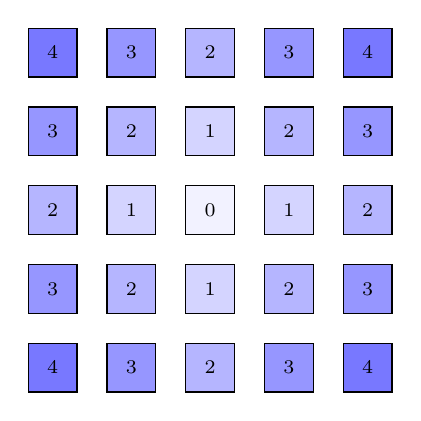
\begin{tikzpicture}[cell/.style={draw, minimum size=0.62cm, font=\scriptsize}]
        \foreach \r in {0,...,4} \foreach \c in {0,...,4} {
          \pgfmathtruncatemacro{\d}{abs(\r-2)+abs(\c-2)}
          \node[cell, fill=blue!\the\numexpr 5+12*\d\relax] at (\c,-\r) {\d};
        }
      \end{tikzpicture}
      \end{center}
      \scriptsize the number is the distance from the centre
    \end{column}
    \begin{column}{0.54\textwidth}
      \begin{itemize}\small
        \item Start at the source: enqueue it, distance 0.
        \item Repeat: \texttt{dequeue} a cell, enqueue every unvisited neighbour with distance $+1$.
        \item BFS visits all cells at distance 0, then 1, then 2, \dots: \hRemark{the queue is the frontier}.
        \item The first time the target is dequeued, its distance is the shortest one.
        \item Uses: shortest path in a maze, social networks, web crawlers, flood fill.
      \end{itemize}
    \end{column}
  \end{columns}
\end{frame}
% ~~~~~~~~~~~~~~~~~~~~~~~~~~~~~~~~~~~~~~ A frm

% ~~~~~~~~~~~~~~~~~~~~~~~~~~~~~~~~~~~~~~ V
\subsection[Buffers]{Buffers and scheduling}
% ~~~~~~~~~~~~~~~~~~~~~~~~~~~~~~~~~~~~~~ A




% ~~~~~~~~~~~~~~~~~~~~~~~~~~~~~~~~~~~~~~ V frm
\begin{frame}[t,fragile] \frametitle{Buffers and scheduling}
  \begin{columns}[T]
    \begin{column}{0.44\textwidth}
      \begin{center}
      \begin{tikzpicture}[box/.style={draw, thick, rounded corners=2pt, minimum height=0.8cm, font=\scriptsize}, node distance=0.55cm]
        \node[box, fill=colorHead!60] (p) {producer};
        \node[box, fill=colorUsed!50, right=of p] (q) {queue};
        \node[box, fill=colorTop!50, right=of q] (c) {consumer};
        \draw[-latex, thick] (p) -- (q);
        \draw[-latex, thick] (q) -- (c);
      \end{tikzpicture}
      \end{center}
      \scriptsize the producer and the consumer work at different speeds
    \end{column}
    \begin{column}{0.54\textwidth}
      \begin{itemize}\small
        \item \textbf{Producer/consumer buffer}: the queue absorbs a fast producer or a slow consumer.
        \item \textbf{Round-robin scheduling}: the operating system keeps the ready processes in a queue.
        \item \textbf{Network and sound buffers}: a bounded queue smooths a burst.
        \item \textbf{Message queues} (Kafka, RabbitMQ): queues between programs, on different machines.
        \item \textbf{Printers, call centres, ticket counters}: the same idea without a computer.
      \end{itemize}
    \end{column}
  \end{columns}
\end{frame}
% ~~~~~~~~~~~~~~~~~~~~~~~~~~~~~~~~~~~~~~ A frm




% ~~~~~~~~~~~~~~~~~~~~~~~~~~~~~~~~~~~~~~ V frm
\begin{frame}[t,fragile] \frametitle{More uses}
  \begin{columns}[T]
    \begin{column}{0.48\textwidth}
      \begin{itemize}
        \item \textbf{Level-order traversal} of a tree: visit the root, then its children, then theirs.
        \item \textbf{Palindrome}: a deque, take one character from each end (examples deck).
        \item \textbf{Josephus problem}: people in a circle, every $k$-th leaves.
        \item \textbf{Hot potato}: pass an object around a circle.
      \end{itemize}
    \end{column}
    \begin{column}{0.48\textwidth}
      \begin{itemize}
        \item \textbf{Sliding-window maximum}: a deque keeps the candidates of each window.
        \item \textbf{Undo history with a limit}: keep the last $n$ actions.
        \item \textbf{Web server}: requests wait in a queue for a worker thread.
        \item \textbf{Simulation}: bank, supermarket, hospital: measure the waiting time.
      \end{itemize}
    \end{column}
  \end{columns}
  \vspace{0.6em}
  \begin{block}{The pattern}
    \small Whenever the \emph{order of arrival} must be preserved, a queue is the natural container.
  \end{block}
\end{frame}
% ~~~~~~~~~~~~~~~~~~~~~~~~~~~~~~~~~~~~~~ A frm

% ~~~~~~~~~~~~~~~~~~~~~~~~~~~~~~~~~~~~~~ V
\hSection[Java]{Queues in Java}
% ~~~~~~~~~~~~~~~~~~~~~~~~~~~~~~~~~~~~~~ A




% ~~~~~~~~~~~~~~~~~~~~~~~~~~~~~~~~~~~~~~ V frm
\begin{frame}[t,fragile] \frametitle{Which class?}
  \begin{center}\footnotesize
  \begin{tabular}{@{}lL{0.16\textwidth}L{0.44\textwidth}@{}}
    \toprule
    \textbf{Class (in \texttt{java.util})} & \textbf{Since} & \textbf{Note} \\
    \midrule
    \hCode{ArrayDeque}           & Java 6 (2006) & \hRemark{recommended}: a growing circular array; also a \texttt{Deque} \\
    \hCode{LinkedList}           & Java 1.2      & a linked list; also a \texttt{Deque} \\
    \hCode{PriorityQueue}        & Java 5        & \hRemark{not FIFO}: the smallest element leaves first \\
    \hCode{ArrayBlockingQueue}   & Java 5        & bounded, waits when full or empty \\
    \hCode{ConcurrentLinkedQueue}& Java 5        & unbounded, lock-free, for many threads \\
    \bottomrule
  \end{tabular}
  \end{center}
  \vspace{0.3em}
  \begin{itemize}\small
    \item The interface \texttt{java.util.Queue} has \texttt{offer}, \texttt{poll}, \texttt{peek}: they return \texttt{false}/\texttt{null} instead of throwing.
    \item \texttt{add}, \texttt{remove}, \texttt{element} are the same operations, but they \textbf{throw} on failure.
    \item There is no \texttt{java.util.Queue} class: it is an interface. \texttt{ArrayDeque} is the usual implementation.
  \end{itemize}
\end{frame}
% ~~~~~~~~~~~~~~~~~~~~~~~~~~~~~~~~~~~~~~ A frm




% ~~~~~~~~~~~~~~~~~~~~~~~~~~~~~~~~~~~~~~ V frm
\begin{frame}[t,fragile] \frametitle{Trying it: \texttt{jshell}}
  \small Open a terminal (\win: \emph{Command Prompt}; \mac: \emph{Terminal}) and type \texttt{jshell}.
  The same lines, saved as \texttt{try.jsh}:
  \lstcode[basicstyle=\ttfamily\tiny, numbers=none]{codeoutput/JShell/try.jsh}{Java}

  \lstterminal[basicstyle=\ttfamily\footnotesize]{codeoutput/JShell.txt}

  \vspace{0.1em}
  \small \texttt{ArrayDeque} prints from the \textbf{front}: \texttt{[10, 20, 30]}.
\end{frame}
% ~~~~~~~~~~~~~~~~~~~~~~~~~~~~~~~~~~~~~~ A frm

% ~~~~~~~~~~~~~~~~~~~~~~~~~~~~~~~~~~~~~~ V
\hSection[Summary]{Summary}
% ~~~~~~~~~~~~~~~~~~~~~~~~~~~~~~~~~~~~~~ A




% ~~~~~~~~~~~~~~~~~~~~~~~~~~~~~~~~~~~~~~ V frm
\begin{frame}[t,fragile] \frametitle{Big ideas}
  \begin{itemize}
    \item A queue is \textbf{FIFO}: insert at the rear, remove at the front.
    \item ADT: \texttt{enqueue}, \texttt{dequeue}, \texttt{peek}, \texttt{isEmpty}, \texttt{size}; errors are \emph{overflow} and \emph{underflow}.
    \item With an array: two indices, \texttt{head} and \texttt{tail}, and a \textbf{circular} array so the free slots at the front are reused.
    \item Empty or full? Keep a \texttt{size} counter (or one slot free). Do not guess from the two indices alone.
    \item Every operation is $O(1)$; a growing array doubles its capacity, $O(1)$ amortized.
    \item Uses: printers, buffers, scheduling, breadth-first search, simulations, message queues.
    \item In Java: \texttt{ArrayDeque} implements \texttt{Queue}; \texttt{PriorityQueue} is \emph{not} FIFO.
  \end{itemize}
\end{frame}
% ~~~~~~~~~~~~~~~~~~~~~~~~~~~~~~~~~~~~~~ A frm




% ~~~~~~~~~~~~~~~~~~~~~~~~~~~~~~~~~~~~~~ V frm
\begin{frame}[t,fragile] \frametitle{Check yourself}
  \begin{enumerate}\small
    \item After \texttt{enqueue(1), enqueue(2), dequeue(), enqueue(3), peek()}, what is returned and what is left?
    \item A circular array has capacity 8, \texttt{head = 6}, \texttt{size = 4}. Which indices hold the elements?
    \item Why does a circular queue keep a \texttt{size} counter (or one free slot)?
    \item Why is \texttt{dequeue} with shifting $O(n)$ and with two indices $O(1)$?
    \item Why does a growing queue double its array instead of adding one slot?
    \item A queue holds 2 elements. Can \texttt{head == tail}? When?
    \item Which Java class would you use for FIFO, and which for ``smallest first''?
  \end{enumerate}
\end{frame}
% ~~~~~~~~~~~~~~~~~~~~~~~~~~~~~~~~~~~~~~ A frm




% ~~~~~~~~~~~~~~~~~~~~~~~~~~~~~~~~~~~~~~ V frm
\begin{frame}[t,fragile]
	\begin{center}
		\vspace{4cm}
		\hRemark{\Huge Questions?}
	\end{center}
\end{frame}
% ~~~~~~~~~~~~~~~~~~~~~~~~~~~~~~~~~~~~~~ A frm




\end{document}
